\chapter{Trigonometry Review}
\label{chap:TR}
Further reading: \texttt{Chen \& Duong ``mtfym01.pdf''},\, \url{http://goo.gl/wyojl}

\begin{bigideas}{sec:TR Big Ideas}
\begin{itemize}
  \item Radians and arc length are interrelated. There are $2\pi$ radians
  in a circle.
  \item An angle subtended by $\theta$ will have arc length $\theta$.
  \item $\cos(\theta) = y$-ordinate, $\sin(\theta) = x$-ordinate
  \item $\tan(\theta) = \frac{\sin(\theta)}{\cos(\theta)} = \frac{y}{x}$
  \item \nameref{sec:TR Pythagorean Identities} (page \pageref{sec:TR
  Pythagorean Identities}) are worth learning!
\end{itemize}
\end{bigideas}

\section{Radian \& Arc Length}
\label{sec:TR Radian and Arc Length}
Further reading: \texttt{Chen \& Duong ``mtfym01.pdf'' pp 1-2},\, \url{http://goo.gl/wyojl}

Radians and arc length are interrelated. There are $2\pi$ radians in a circle,
that is a semi-circle has about $3.14$ radians ($\pi$ radians to be exact).

In areas of maths, science and engineering radians are used as the main unit of
measurement of angles rather than degrees, as such it can be handy to know how
to convert between the two units.

\begin{align}
  \text{degrees} & = \text{radians} \times \frac{180}{\pi} \\[0.5cm]
  \text{radians} & = \text{degrees} \times \frac{\pi}{180}
\end{align}

Aside from the conversion formula, it is also useful to remember the following
special values:

\begin{align}
  \frac{\pi}{6} & = 30\ndeg \\[0.5cm]
  \frac{\pi}{4} & = 45\ndeg \\[0.5cm]
  \frac{\pi}{3} & = 60\ndeg \\[0.5cm]
  \frac{\pi}{2} & = 30\ndeg \\[0.5cm]
  \pi           & = 180\ndeg \\[0.5cm]
  2\pi &= 360\ndeg
\end{align}

\section{The Unit Circle}
\label{sec:TR Unit Circle}

In high school we learned that trigonometry was about angles of triangles, and
while this remains true, we look at it in the context of circles. Consider a
special circle called \emph{the unit circle}. See (ref fig \ref{fig:UnitCircle}
page \pageref{fig:UnitCircle}). If we run a vertical line from each point in the
unit circle to the line $y=0$, the triangle is formed.
\begin{center}
% Unit circle
% Author: Supreme Aryal
% A unit circle with cosine and sine values for some
% common angles.
\begin{figure}[!htb]
\label{fig:UnitCircle}
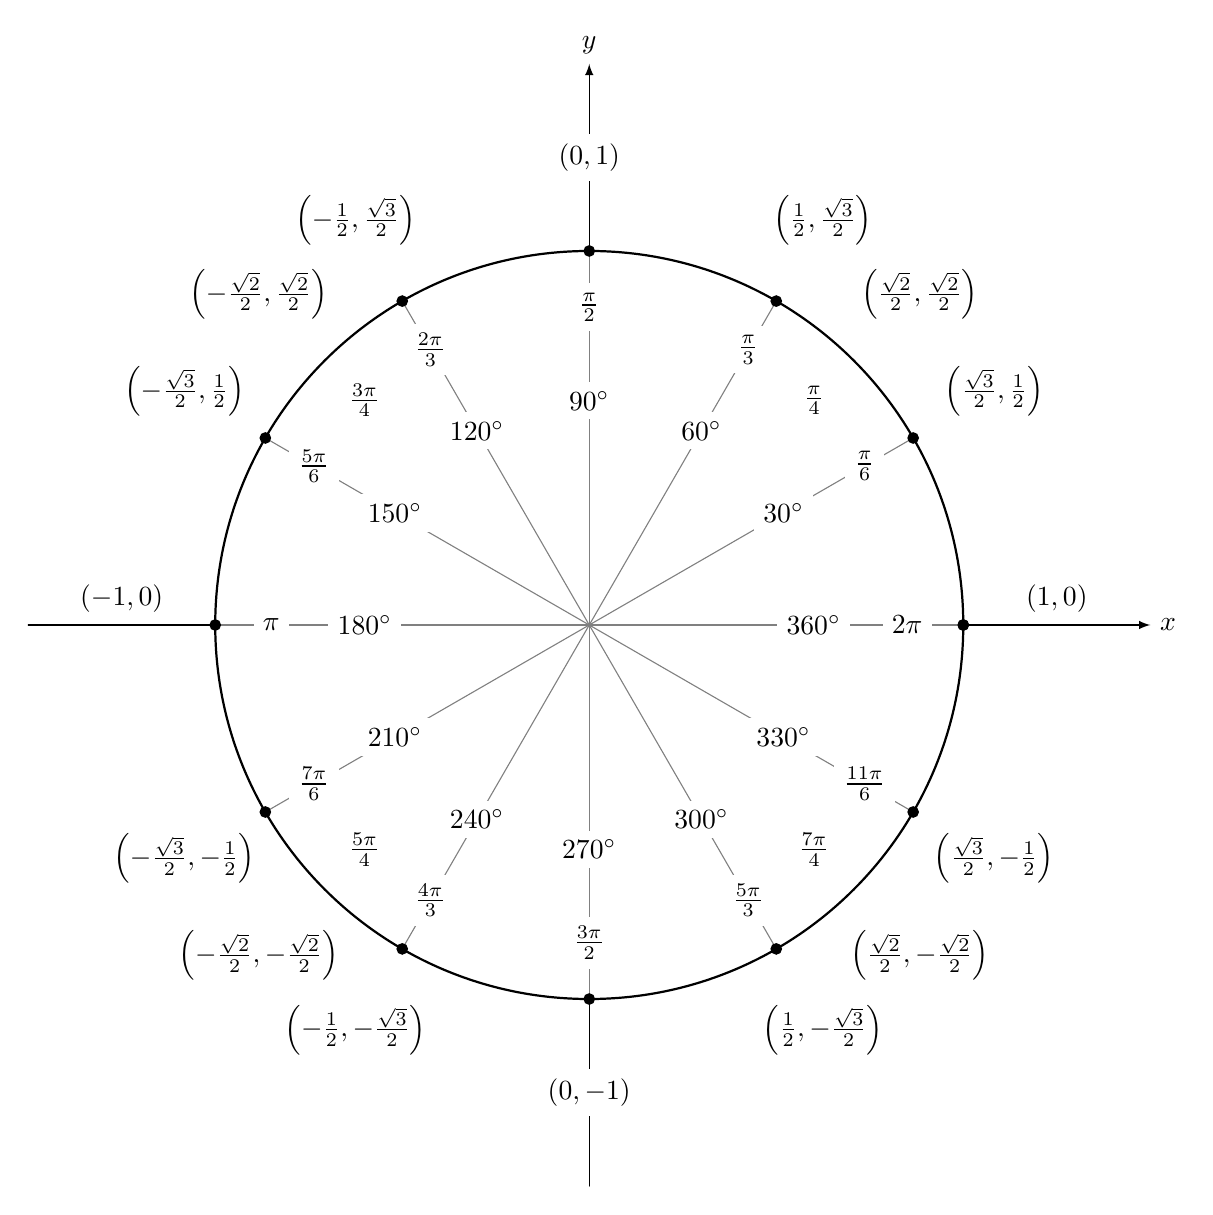
\begin{tikzpicture}[scale=4.75,cap=round,>=latex]
    % draw the coordinates
    \draw[->] (-1.5cm,0cm) -- (1.5cm,0cm) node[right,fill=white] {$x$};
    \draw[->] (0cm,-1.5cm) -- (0cm,1.5cm) node[above,fill=white] {$y$};

    % draw the unit circle
    \draw[thick] (0cm,0cm) circle(1cm);

    \foreach \x in {0,30,...,360} {
      % lines from center to point
      \draw[gray] (0cm,0cm) -- (\x:1cm);
      % dots at each point
      \filldraw[black] (\x:1cm) circle(0.4pt);
      % draw each angle in degrees
      \draw (\x:0.6cm) node[fill=white] {$\x^\circ$};
    }

    % draw each angle in radians
    \foreach \x/\xtext in {
      30/\frac{\pi}{6},
      45/\frac{\pi}{4},
      60/\frac{\pi}{3},
      90/\frac{\pi}{2},
      120/\frac{2\pi}{3},
      135/\frac{3\pi}{4},
      150/\frac{5\pi}{6},
      180/\pi,
      210/\frac{7\pi}{6},
      225/\frac{5\pi}{4},
      240/\frac{4\pi}{3},
      270/\frac{3\pi}{2},
      300/\frac{5\pi}{3},
      315/\frac{7\pi}{4},
      330/\frac{11\pi}{6},
      360/2\pi
    }
    \draw (\x:0.85cm) node[fill=white] {$\xtext$};

    \foreach \x/\xtext/\y in {
      % the coordinates for the first quadrant
      30/\frac{\sqrt{3}}{2}/\frac{1}{2},
      45/\frac{\sqrt{2}}{2}/\frac{\sqrt{2}}{2},
      60/\frac{1}{2}/\frac{\sqrt{3}}{2},
      % the coordinates for the second quadrant
      150/-\frac{\sqrt{3}}{2}/\frac{1}{2},
      135/-\frac{\sqrt{2}}{2}/\frac{\sqrt{2}}{2},
      120/-\frac{1}{2}/\frac{\sqrt{3}}{2},
      % the coordinates for the third quadrant
      210/-\frac{\sqrt{3}}{2}/-\frac{1}{2},
      225/-\frac{\sqrt{2}}{2}/-\frac{\sqrt{2}}{2},
      240/-\frac{1}{2}/-\frac{\sqrt{3}}{2},
      % the coordinates for the fourth quadrant
      330/\frac{\sqrt{3}}{2}/-\frac{1}{2},
      315/\frac{\sqrt{2}}{2}/-\frac{\sqrt{2}}{2},
      300/\frac{1}{2}/-\frac{\sqrt{3}}{2}
    }
    \draw (\x:1.25cm) node[fill=white] {$\left(\xtext,\y\right)$};

    % draw the horizontal and vertical coordinates
    % the placement is better this way
    \draw (-1.25cm,0cm) node[above=1pt] {$(-1,0)$}
          (1.25cm,0cm)  node[above=1pt] {$(1,0)$}
          (0cm,-1.25cm) node[fill=white] {$(0,-1)$}
          (0cm,1.25cm)  node[fill=white] {$(0,1)$};
  \end{tikzpicture}
\caption{The Unit Circle, courtesy of Supreme Ayal, TiKZ Examples \cite{HTrCS}}
\end{figure}
\end{center}

\section{Trigonometric Functions}
\label{sec:TR Trigonometric Functions}
Further reading: \texttt{Chen \& Duong ``mtfym01.pdf'' pp 2-4},\, \url{http://goo.gl/wyojl}

Looking at the unit circle, an angle is defined by the two points, the first
at the origin $(0,0)$, the second is $(\cos\theta), \sin\theta)$. That is to say

\begin{align}
  x = \cos\theta
  & \quad \text{and} \quad &
  y = \sin\theta 
\end{align}
Additionally, we can define $\tan\theta$:
\begin{align}
  \tan\theta = \frac{\sin\theta}{\cos\theta} = \frac{y}{x}
\end{align}
Finally there are the inverse trigonometric functions:
\begin{align}
  \sec\theta = \frac{1}{\cos\theta} = \frac{1}{x}
  & \quad \text{and} \quad &
  \csc\theta = \frac{1}{\sin\theta} = \frac{1}{y}
\end{align}
\begin{align}
  \cot\theta = \frac{\cos\theta}{\sin\theta} = \frac{x}{y}
\end{align}
Note: $\tan\theta$ and $\sec\theta$ are defined only when $\cos\theta \neq 0$
and $\cot\theta$ and $\csc\theta$ are defined only when $\sin\theta \neq 0$.

\section{Pythagorean Identities}
\label{sec:TR Pythagorean Identities}
Further reading: \texttt{Chen \& Duong ``mtfym01.pdf'' pp 4-5},\, \url{http://goo.gl/wyojl}

\begin{align}
  \cos^{2}\theta + \sin^{2}\theta &= 1 \label{eq:pythagIdent}
\intertext{By dividing \ref{eq:pythagIdent} by $\cos^{2}\theta$ we get:}
  1 + \tan^{2}\theta &= \sec^{2}\theta
\intertext{By dividing \ref{eq:pythagIdent} by $\sin^{2}\theta$ we get:}
  1 + \cot^{2}\theta &= \csc^{2}\theta
\end{align}

\section{Properties of Trigonometric Functions}
\label{sec:TR Trigonometric Functions - Properties}
Further reading: \texttt{Chen \& Duong ``mtfym01.pdf'' pp 5-10},\, \url{http://goo.gl/wyojl}

\subsection{Properties of $\sin\theta$}
\label{subsec:TR Trigonometric Functions - sin}
\begin{align}
  \cos(\theta + 2\pi) & = \cos\theta \\
  \cos(-\theta) & = -\cos\theta \\
  \cos(\theta + \pi) & = -\cos\theta \\
  \cos(\pi - \theta) & = \cos\theta
\end{align}
\begin{center}
\begin{figure}[!htb]
\label{fig:cosx}
\begin{tikzpicture}
  \draw[very thin, color=lightgray] (-6.28, -1.5) grid (6.28, 1.5);
  \draw[<->] (-6.28,0) -- (6.28,0);
  \draw[<->] (0,-1.5) -- (0,1.5);
  \draw[smooth,color=nicered]
    plot[thick,id=cosx,samples=200,domain=-6.28:6.28]
    function{cos(x)}
    node at (2.5,0.5) {$f(x) = \cos\theta$}; 
\end{tikzpicture}
\caption{$f(x) = \cos\theta$}
\end{figure}
\end{center}

\subsection{Properties of $\cos\theta$}
\label{subsec:TR Trigonometric Functions - cos}
\begin{align}
  \sin(\theta + 2\pi) & = \sin\theta \\
  \sin(-\theta) & = -\sin\theta \\
  \sin(\theta + \pi) & = -\sin\theta \\
  \sin(\pi - \theta) & = \sin\theta
\end{align}
\begin{center}
\begin{figure}[!htb]
\label{fig:sinx}
\begin{tikzpicture}
  \draw[very thin, color=lightgray] (-6.28, -1.5) grid (6.28, 1.5);
  \draw[<->] (-6.28,0) -- (6.28,0);
  \draw[<->] (0,-1.5) -- (0,1.5);
  \draw[smooth,color=nicered]
    plot[thick,id=sinx,samples=200,domain=-6.28:6.28]
    function{sin(x)};
  \draw[color=black]
    node at (1,-0.5) {$f(x) = \sin\theta$}; 
\end{tikzpicture}
\caption{$f(x) = \sin\theta$}
\end{figure}
\end{center}

\subsection{Properties of $\tan\theta$}
\label{subsec:TR Trigonometric Functions - tan}
\begin{align}
  \tan(\theta + \pi) & = \tan\theta \\
  \tan(-\theta) & = -\tan\theta \\
  \tan(\pi - \theta) & = -\tan\theta
\end{align}
\begin{center}
\begin{figure}[!htb]
\label{fig:tanx}
\begin{tikzpicture}
  \clip(-6.28,-4.5) rectangle (6.28,4.5);
  \draw[very thin, color=lightgray] (-6.28, -4.5) grid (6.28, 4.5);
  \draw[<->] (-6.28,0) -- (6.28,0);
  \draw[<->] (0,-4.5) -- (0,4.5);
  \draw[smooth,color=nicered]
    plot[thick,id=tanx,samples=200,domain=-6.28:6.28]
    function{tan(x)};
  \draw[color=black]
    node at (3,1.5) {$f(x) = \tan\theta$}; 
  \clip(-6.28,-4.5) rectangle (6.28,4.5);
\end{tikzpicture}
\caption{$f(x) = \tan\theta$}
\end{figure}
\end{center}

\section{Trigonometric Identities}
\label{sec:TR Trigonometric Identities}
Further reading: \texttt{Chen \& Duong ``mtfym01.pdf'' pp 11},\, \url{http://goo.gl/wyojl}

\subsection{Sine Rule}
\label{subsec:TR Trigonometric Identities - Sine Rule}

\begin{align}
  \frac{a}{\sin(A)} \quad = \quad \frac{b}{\sin(B)} \quad = \quad \frac{c}{\sin(C)}
\end{align}

\subsection{Cosine Rule}
\label{subsec:TR Trigonometric Identities - Cosine Rule}

\begin{align}
  a^2 &= b^2 + c^2 - 2bc\cos(A) \\[0.5cm]
  b^2 &= a^2 + c^2 - 2ac\cos(B) \\[0.5cm]
  c^2 &= a^2 + b^2 - 2ab\cos(C)
\end{align}

\subsection{Angle Sum \& Difference Identities}
\label{subsec:TR Trigonometric Identities - Angle Sum Identities}
Further reading: \texttt{Chen \& Duong ``mtfym01.pdf'' pp 12},\, \url{http://goo.gl/wyojl}

\begin{align}
  \sin(A \pm B) &= \sin(A)\cos(\B) \pm \cos(A)\sin(B) \\[0.5cm]
  \cos(A \pm B) &= \cos(A)\cos(\B) \mp \sin(A)\sin(B)
\end{align}

\subsubsection{Double Angle Identity}
\label{subsubsec:TR Trigonometric Identities - Angle Sum Identities - Double Angle Identity}
Further reading: \texttt{Chen \& Duong ``mtfym01.pdf'' pp 12},\, \url{http://goo.gl/wyojl}

\begin{align}
  \sin(2\theta) & = 2\sin(\theta)\cos(\theta) \\[0.5cm]
  \cos(2\theta) & = \cos^2(\theta) - \sin^2(\theta) \\
                & = 1 - 2\sin^(\theta) \\
                & = 2c\cos^2(\theta) - 1
\end{align}

\subsubsection{Half Angle Identity}
\label{subsubsec:TR Trigonometric Identities - Angle Sum Identities - Half Angle Identity}
Further reading: \texttt{Chen \& Duong ``mtfym01.pdf'' pp 13-15},\, \url{http://goo.gl/wyojl}

\begin{align}
  \sin^2\left(\frac{\theta}{2}\right) = \frac{1 - \cos(\theta)}{2} \\[0.5cm]
  \cos^2\left(\frac{\theta}{2}\right) = \frac{1 + \cos(\theta)}{2}
\end{align}